%This new document is an article
\documentclass[12pt,letterpaper]{article}


% Some useful packages
\usepackage{caption} % for the figure captions
\usepackage[osf]{mathpazo} % a nicer font
\usepackage{natbib} % this is a package for the citation formats
\usepackage{amsmath} % package for equations
\usepackage{url} % package for urls
\usepackage{hyperref} % for hyperlinks
\usepackage{graphicx} % for the figures
\pagenumbering{arabic} % stating the page number type


% Let's start
\begin{document}


%---------------------------------------------
%
%       HEADER - title and abstract
%
%---------------------------------------------

% Always useful to have the date, but let's put it on the right
\begin{flushright}
Version dated: \today
\end{flushright}

\bigskip % Some space between the date and the title

\begin{center} % Starting the header in the center

\noindent{\Large{\textbf{My paper written in latex.}}} % The title in large and bold with not indent
\bigskip

\noindent{Thomas Guillerme$^1$$^,$$^*$ and My Coauthor$^1$$^,$$^2$}\\ % here "^" indicates the indices and "$" groups the indices and the number.
\noindent{\small{\textit{
$^1$Department of Life Sciences, Imperial College London, Silwood Campus, United Kingdom\\ % the double backslash (\\) is a short cut for indicating a new line.
$^2$Some other place in some other country\\
}}} % Don't forget to close the curly brackets!
\end{center}
\noindent * \textbf{Corresponding author.} \textit{Department of Life Sciences, Imperial College London, Silwood Campus, Buckhurst Road, Ascot SL5 7PY, United Kingdom; E-mail: t.guillerme@imperial.ac.uk.}

\bigskip

\begin{abstract} % This is obvious
Some short abstract here
\end{abstract}

\noindent Key words: Total Evidence method, data structure, phylogenetic, fossil, topology.

\bigskip

%---------------------------------------------
%
%       PAPER - here it comes
%
%---------------------------------------------
\newpage 
\section{Introduction}
Let's start with a first sentence. And then get some cites to support it \citep[e.g ][]{Cooper2008,Brazeau2011,harrisonamong-character2014}. % There are several format for citing, here \citep cites with parenthesis.

\section{Material and Methods}
\subsection{Material}
I got my data from \cite{picante}. % here the cite format will be just author (year)

\subsection{Methods}
\label{methods} % Creating a link to this section (see discussion)
\texttt{R} is awesome for doing some analysis \citep{R}. %Note that \texttt{} is used for writing in courier font.
And it can use pretty sophisticate equations like the Mind Blowing Metric Quotient (MBMQ):
  \begin{equation}
  \label{equation}
    \text{MBMQ}=\frac{\sum{observations}}{n}
  \end{equation}
where \textit{n} is the total number of \textit{observations}.

\section{Results}
Check this out: I made a table and a figure!

\begin{table}[!htpb] % Starting a table section; [!htpb] forces the table to appear in this part of the pdf
\caption{This table doesn't make much sense but some values are highlighted so that's cool.} % The table caption
\label{my_table}
\centering % We want our table centered
\begin{tabular}{c|lr|c} % tabular designate the actual table with the letters being the number and type of columns (c for center; l for left; and r for right) and | if you want to separate columns by a solid line
   & A & B & C \\ % & separates the columns. Note that the first column is left empty (starting directly with &) and \\ ends the rows
   \hline % for a solid horizontal line
  exp1 & 0.1 & 0.2 & 0.3 \\
  exp2 & 0.4 & 0.5 & \textbf{0.05} \\
  exp3 & bla$^1$ & bli & blo \\
\end{tabular} \\
   \small{$^1$ And we can even add footnotes! How awesome!}
\end{table}

\begin{figure}[!htpb]
\centering
    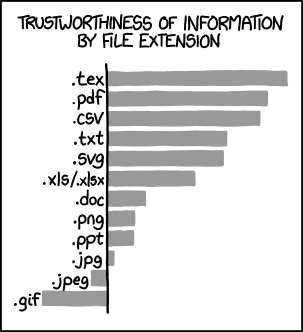
\includegraphics{file_extension_xkcd_1301.png} % The link to the figure
\caption{Some nice information from http://xkcd.com/1301/ (CC-BY NC 2.5)} % The caption
\label{my_figure}
\end{figure}

\newpage % Just to start the discussion in a new page

\section{Discussion}
We can now link to Table \ref{my_table} or Figure \ref{my_figure}.\ref{my_figure}
But it is also possible to refer to equation \ref{equation} or the section \ref{methods}.
Try adding more elements or shuffle them around to see that the links will automatically update!
Of course, real manuscripts are more complex (more authors, more odd things and more journal requirements, see \href{https://github.com/TGuillerme/Total_Evidence_Method-Missing_data/blob/master/Manuscript/TEM_revised_manuscrip_highlithed.tex}{this real example}). 

\section{Acknowledgements}
Thanks folks

\bibliographystyle{sysbio}
\bibliography{References}



%END
\end{document}
